\section{Preliminary Study}

\begin{figure}[!t]

  \centering
  \hspace*{-1em}

  \begin{minipage}{4in}
    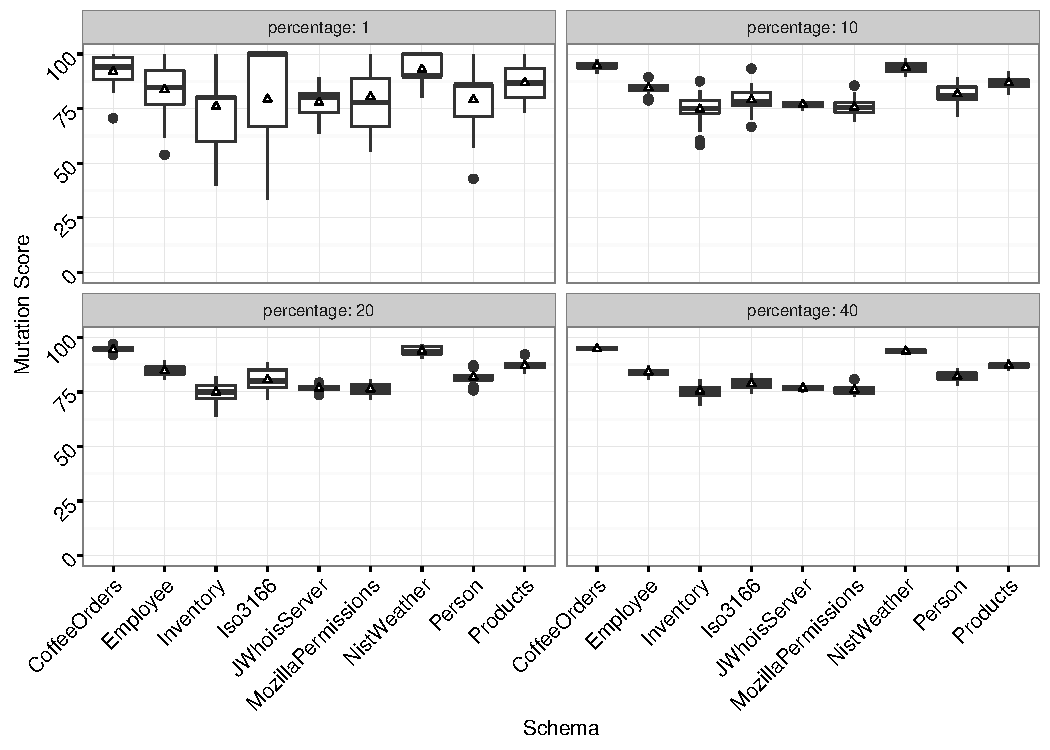
\includegraphics[scale = 0.5]{graphs/schema_vs_ms.pdf}
  \end{minipage}

  \caption{\label{fig:graph}Graph displaying mutation scores for database schemas.}

  \vspace{-1.8em}

\end{figure}


% GMK NOTE: All of this content is really about the design of the experiments and thus it has to be integrated into this
% section (currently, this is still rough content).

We chose these nine schemas because they range in triviality. For example, the MozillaPermissions schema contains a
single constraint, where as the JWhoisServer schema has a total of 50 constraints. This allowed us to evaluate the
policy recommendations made based on the effectiveness of reduction techniques analysed by \mr~for schemas of varying
complexities.

Where Wong and Mathur in their studies~\cite{mathur1994empirical, wong1993mutation} conducted experiments using mutant
sampling with $x$ from $10\%$ to $40\%$ increasing by steps of $5\%$, we chose to analyse $x$ at $1\%$ and then increase
by $10\%$ intervals up to $90\%$. By lowering the granularity of the experiment to $10\%$ intervals instead of $1\%$ or
$5\%$, we reduce the cost of performing retrospective analysis with \mr, while observing similar trends.

